%The introduction is one of the most important pieces of your thesis.  Here is a place for you to introduce the problem(s) on which you have worked and place them in the larger context of your field.  You should aim to ensure that this section is completely understandable to virtually anyone - and certainly anyone with a sophomore-level grasp of physics.  Presumably this will include references to the literature.

%In addition to setting your work into context, a second good idea for your introduction is to give a short outline for what the rest of your thesis will discuss.  This is often done in the closing paragraph(s) of the introduction with sentences like ``In the following chapters \ldots " and ``Chapter 2 discusses \ldots"  Tremendous detail is not required in this outline, but rather just a brief road map for the rest of the document.

\section{Motivations}
Soft Condensed Matter Physics includes the study of colloids, liquid crystals, polymers, complex fluids, rubbers, foams, many biological materials, and - what we devote most of our time to studying in the Jensen lab - gels. From cosmetics to sticky notes, soft solids are ubiquitous in everyday life and are of growing interest due to their unique properties compared to traditional (hard) engineering materials.  It is important to understand how such ubiquitous materials behave, especially when put under the strains of life. Accordingly, the topic of adhesion and wetting has been studied for hundreds of years, and yet, a discipline with many mysteries still to be explored  \cite{GennesPierre-Gillesde2003Cawp}. 

 
\section{Historical Context}
\subsection{Development of Surface Tension}
Though few people may know the term, surface stress is a familiar concept in everyday phenomena: water droplets bead up into spheres, paperclips can float on water despite being made of dense iron, and water striders navigate the water's surface thanks to their hydrophobic legs. Each of these marvels is a result of \textbf{surface stress},$\Upsilon$, the  energetic cost per unit area to create new surface \cite{cammarata1994surface}. The water strider, for example, exerts a force on the water due to gravity. Because creating new surface costs energy, the water resists deformation, providing a restorative force that effectively balances the insect’s weight to keep it afloat. Likewise, water droplets bead up and liquid surfaces are smooth because $\Upsilon$ acts to minimize the surface-to-volume ratio of the liquid \cite{gibbs1906scientific,GennesPierre-Gillesde2003Cawp}. \todo[inline,color=pink]{de Gennes inspired revisions below}

Let's dissect the example of a water strider (rather than the water strider itself!). Water remains in the liquid phase when the thermal agitations are stronger than the cohesive attractive between the molecules, but not so strong that the water vaporizes. This dense yet disordered state consists of both molecules at the surface and molecules in the bulk. Any given molecule in the bulk is surrounded equally by particles on all sides, resulting in symmetrically balanced forces in all directions. A surface molecule, however, is missing half of these attractions. Thus the cohesive energy per moleculue at the surface is rougly half that of a molecule in the bulk \cite{GennesPierre-Gillesde2003Cawp}. 
\begin{figure}
	\centering
	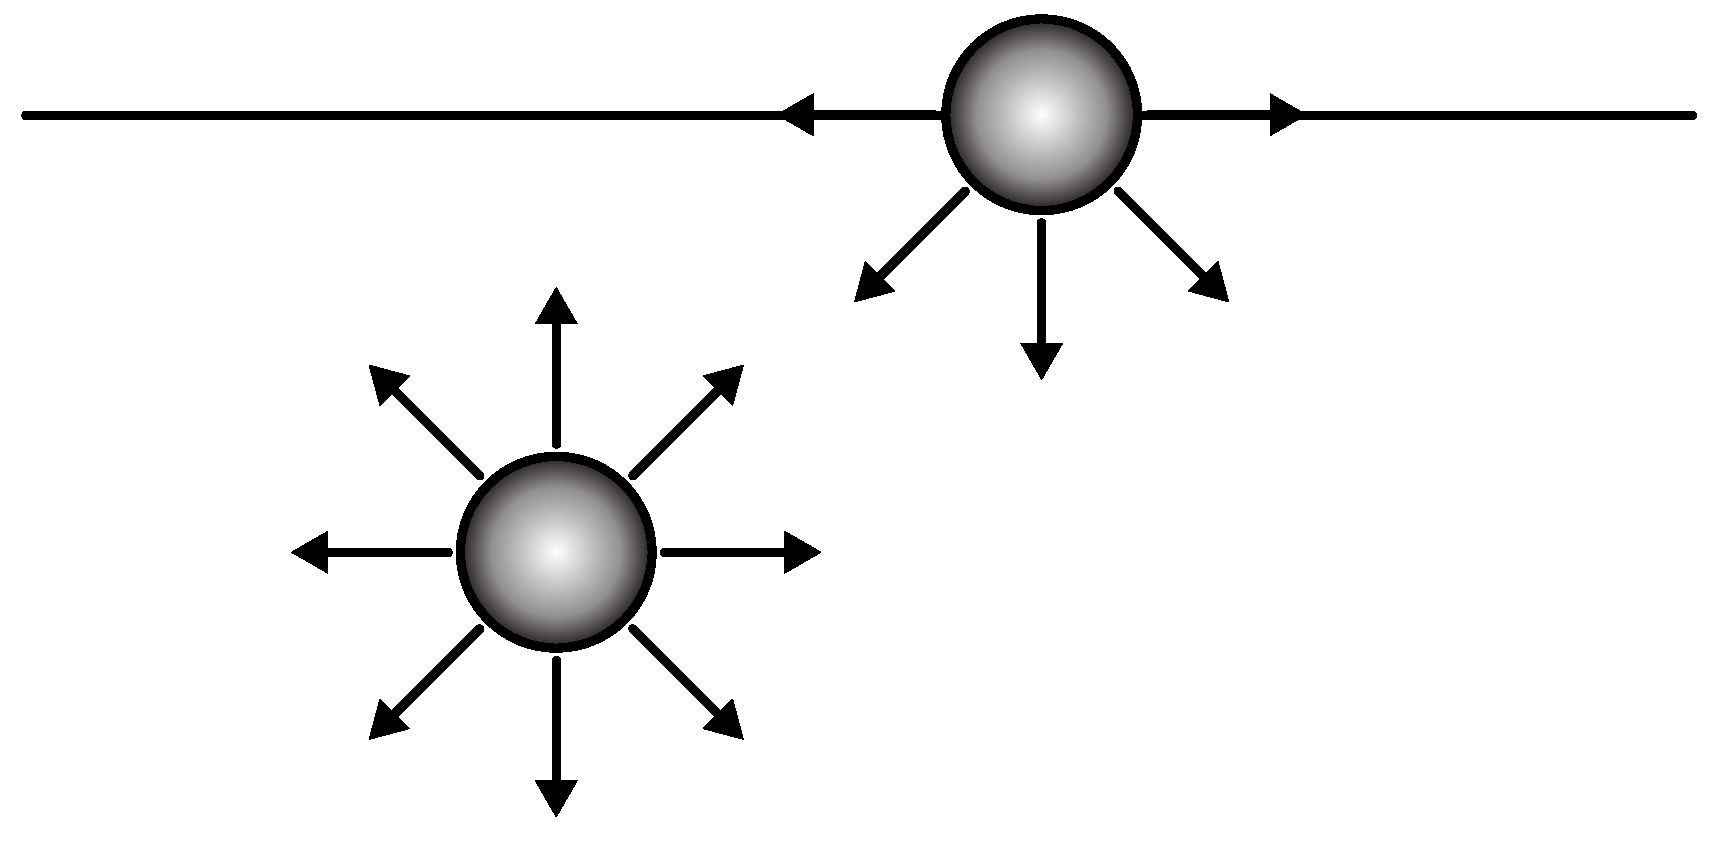
\includegraphics[width=0.7\linewidth]{Chapters/Figures/surface_energy_origin}
	\caption[Surface Free Energy]{A molecule in the bulk has twice as many neighboring molecules than one on the surface, and thus, twice as many neighboring attractions. }
	\label{fig:surfaceenergyorigin}
\end{figure}
The difference in energy between particles in the bulk compared to the surface is known as the \textbf{surface free energy}, $\gamma$, often written as just surface energy. Equivalently, $\gamma$ can also be defined as the reversible work per unit area to create new surface by cutting. This exposes new particles to the surface. When the surface of a fluid is ``stretched,'' however, new atoms or molecules arrive at the surface, maintaining the number of atoms per unit area as a constant value. Therefore, the surface energy is the same as the surface stress for a fluid and equal to a constant value. Because of this, $\gamma$ and $\Upsilon$ have are often referred to interchangeably as \textbf{surface tension}. While conceptually the energetics are similar in liquid materials, the situation becomes more complicated for materials which cannot flow.


%This difference in energy per unit surface area is known as the surface tension. This setup is true not only for fluids, but also for stiff solids. 
%
%The energy associated with particles in the bulk is less than that of the particles at the surface. Molecules beneath the surface are attracted by the particles around them in every direction. In contrast, the particles at the surface are only attracted by the molecules directly adjacent to them. As a result of these less favorable interactions, they are in a state of higher energy compared to molecules in the bulk. The difference in energy between particles in the bulk compared to the surface is known as the \textbf{surface free energy}, $\gamma$, often written as just surface energy. Equivalently, $\gamma$ can also be defined as the reversible work per unit area to create new surface by cutting. This exposes new particles to the surface. When the surface of a fluid is ``stretched,'' however, new atoms or molecules arrive at the surface, maintaining the number of atoms per unit area as a constant value. Therefore, the surface energy is the same as the surface stress for a fluid and equal to a constant value. Because of this, $\gamma$ and $\Upsilon$ have are often referred to interchangeably as \textbf{surface tension}. While conceptually the energetics are similar in liquid materials, the situation becomes more complicated for materials that cannot flow.

\subsection{Surface Tension in Solids}
In metals, the origin of surface stress, on the atomic scale, derives from the crystalline structure. The epitaxial layer, or surface atoms, reside in a lower electron density and therefore a different equilibrium spacing than the bulk. The bulk atoms force the surface atoms to fit into the epitaxial overlayer of the crystalline substrate. As a result, the surface atoms are strained by the bulk, leaving the surface stressed by the underlying lattice \cite{cammarata1994surface}. 

Theoretical calculations for surface stress generally involve the taking the derivative of the predicted surface free energy with respect to strain. Various methods for metals involve calculating the electronic density, the kinetic energy, and the electrostatic exchange-correlation\footnote{Forgoing the independent electron approximation, the electronic exchange is a measure of deflection due to the presence of other electrons} \cite{GURTIN1978431}. 


Experimental measurements of surface stress have been around as early as the 1960's, though measurements of strain-dependent surface stress in stiff materials have only been attempted much more recently and returned scant results \cite{mays1968surface,wasserman1970determination,hanneman1962elastic,martinez1990direct,schell1990mechanical}. Metals are an incredibly useful building tool due to their strength\footnote{Strength: the maximum force per unit area a material can withstand}, but their stiffness\footnote{Stiffness: the material's resistance to deformation via strain} also makes measuring properties as a function of strain severely limited, as most metals will fracture after a few percent strain. For most solids, these surface effects go unnoticed in everyday life due to the overpowering effects of the bulk's elasticity compared to any surface energies. \todo[color=pink]{See Nat Comm 2017 ref 7-12}



\subsection{Surface Stress Effects in Soft Solids}
For solids of small enough size or soft enough composition, the surface energies can compete with or even dominate the effects of the bulk, resulting in strange and counterinruative material properties. For example, the addition of finite, microscopic, liquid droplets in a soft solid actually stiffens the material \cite{style2015stiffening}. While removing material affects the elastic stiffness, it also increases the surface area. At length scales where surface effects dominate, this increase in surface area has a greater energetic cost, and thus leads to a solid of increased stiffness. Further, surface stresses can drive liquid-like instabilities in soft solids, including rounding out sharp corners \cite{mora2015softening} and solid-cylinder version of the Plateau-Rayleigh instability \cite{mora2010capillarity}.
\todo[inline,color=pink]{Add a sentence or two about adhesion \cite{style2013surface,xu2017direct,Jensen2019SoftMatter,Jensen2017PhysRevX}}

Early observations of $ \Upsilon $ in soft solids came from considering the wetting behavior of liquid droplets on soft solid surfaces \cite{xu2017direct,jerison2011deformation,style2013universal,xu2018surface}. The traditional Young-Dupr\'{e} picture of wetting is shown in Figure \ref{fig:three-phase}.
\begin{figure}[h!]
	\centering
	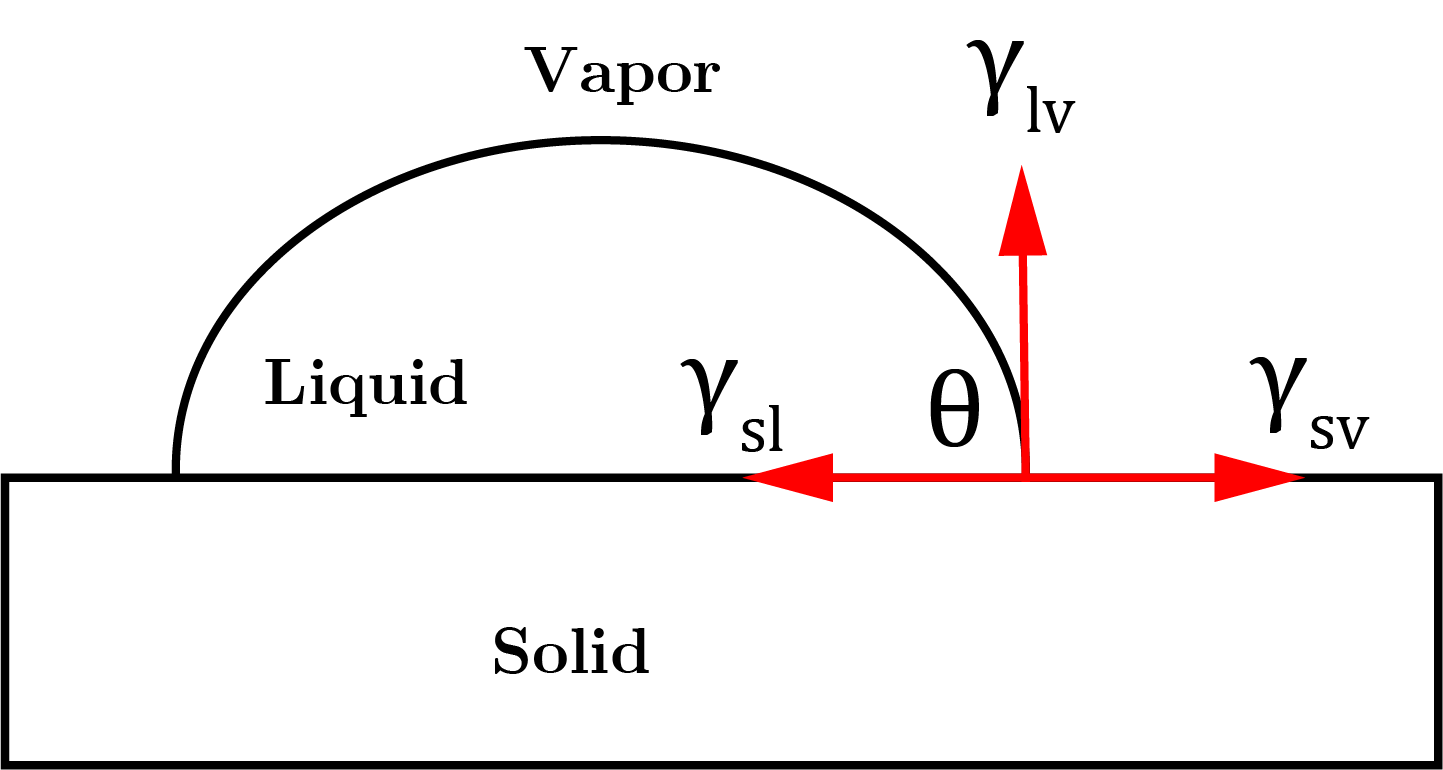
\includegraphics[width=.6\textwidth]{Chapters/Figures/phase_diagram.PNG}
	\caption[Three-Phase Diagram]{Classical Three-Phase Diagram]}
	\label{fig:three-phase} 
\end{figure}
This is clearly an unbalanced force diagram in vertical direction; the only vertical force component drawn is the liquid-vapor surface tension, $ \gamma_{lv} $. The normal force from $\gamma_{lv}$ must be balanced by the elastic substrate's resistance to deformation. Calculating this value, however, is still an open question. According to continuum elastic theory, the stress exerted by $\gamma_{lv}$ on the solid diverges at the contact line \cite{jerison2011deformation}. While Contact Mechanics dates back to the 18th century, seemingly simple problems like a liquid droplet on an elastic surface are still not yet well understood and provide challenging question when inspecting on a small enough scale. 

\begin{figure}[h!]
	\centering
	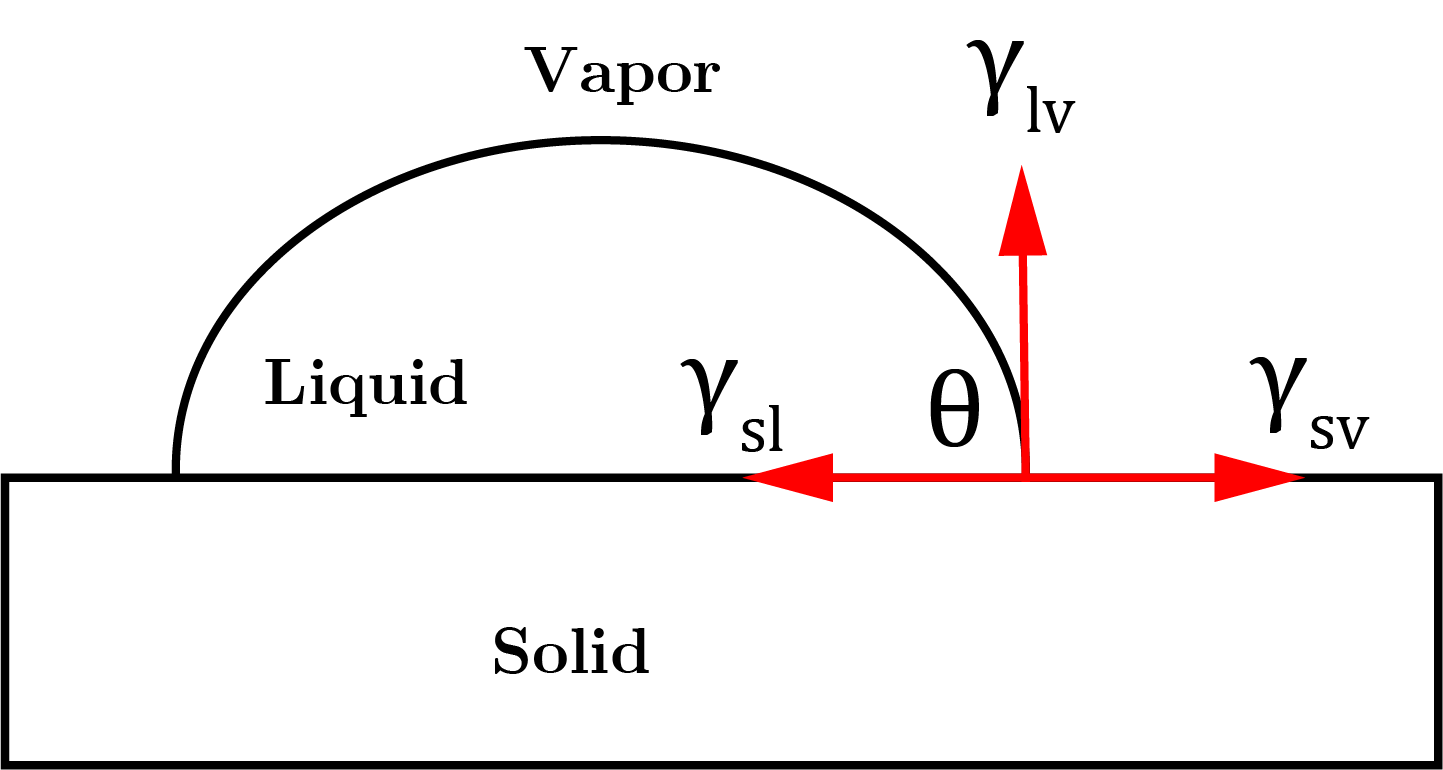
\includegraphics[width=.6\textwidth]{Chapters/Figures/phase_diagram}
%	\caption[Three-Phase Diagram: Zoomed]{When inspected on the microscopic scale, the unbalanced three phase diagram of figure \ref{fig:three-phase} is resolved by the deformation of the substrate.}
	\label{fig:three-phase-zoomed} 
\end{figure}

Jerison et al. 2011 \cite{jerison2011deformation} found modeling the deformation of the elastic substrate due to a liquid droplet fit best with a model that incorporated both the finite thickness and surface tension of the substrate. This new model solved many issues with the previous best solution by Boussinesq: taking into account the finite thickness ensured that the deformations would go to zero far from the contact line, and the substrate's surface tension resolves the single stress singularity, eliminating the divergence of strain and vertical displacement at the origin. This gave us the first method to measure $ \Upsilon $ of a solid directly, tackling a long-standing problem in materials science.
%Note to KEJ: I re-read Jerison 2011. I misread it the first time. In doing their calculations, they assumed the contact angle was close to $ 90\deg $, and they assumed $ \gamma_{sl}=\gamma_{sv} $...but their theory doesn't account for contact angles far from $ 90\deg $....which are the instances in which $ \gamma_{sl}\neq \gamma_{sv} $.


\subsection{Direct Measurement of Solid Surface Stresses}
Measuring the surface stresses even in soft solids has proved experimentally challenging over the years \cite{xu2016surface,jensen2015wetting,mondal2015estimation,style2013surface,jagota2012surface,nadermann2013solid,park2014visualization}. A modern method of measuring the deformation of a soft, elastic solid imposed by the liquid droplet in Figure \ref{fig:three-phase} was introduced by Jerison in 2011 \cite{jerison2011deformation} and later utilized by Style \emph{et al.} in 2013 \cite{style2013universal}. They measured the 3-phase contact line geometry in figure \ref{fig:three-phase} without requiring any prior knowledge about the bulk elastic properties of the substrate material. 

While this technique is effective, it is limited in its applications due to material properties. The method only works for immiscible fluids such that the gel does not absorb the surface droplets. Furthermore, the fluid must also have a low volatility; otherwise, the droplet would begin to evaporate while waiting for the surface deformations to settle. Since then, other methods have been developed, including an adhesion-based technique developed by Style \textit{et al.} in 2013 \cite{style2013surface}. Though the measurement is less direct, this adhesion based method does not suffer from the same material limitations and give us another approach to measuring $ \Upsilon $.  


\subsubsection{Puzzling Surface Stress Measurements in Gels}
In contrast to hard materials\todo[color=pink]{weird to say now that Dupre is moved}, it has been widely assumed that surface stress in soft matter would be nearly strain-independent. Gels, for example, while classified as solid, are comprised mainly of fluid (by weight) and exhibit many properties that are more closely associated with liquids. Their rigidity is a result a three-dimensional network of crosslinked polymers which entrap large amounts of liquid throughout\footnote{For a more in depth explanation, see section \ref{section:polychem}} via capillary forces. The result is a solid whose stiffness is determined by the composition and temperature. Because the surface stress in liquids is constant and equal to the surface energy of the substance $(\Upsilon = \gamma)$, it was largely assumed that deforming a gel would not have a significant effect on the surface tension, given that the fluid could flow back to the stretched surface of the gel. Surface stress in soft solids is a topic of growing interest. Unlike in metals, elastocapillary physics plays a crucial role in determining the material's behavioral properties.  

In the following years, further tests of surface stress in soft solids (Table \ref{tab:upsilon_values}) were measured with wildly varying results. It began to become clear that the surface stress of soft solids was not simply that of the fluid phase, and there is more to the mystery. 
\begin{table}[h!]
	\centering
	\begin{tabular}{|l|l|l|l|}
		\hline
		\textbf{Silicone}       & \multicolumn{1}{c|}{\textbf{\begin{tabular}[c]{@{}c@{}}Young's Modulus \\ (kPa)\end{tabular}}} & \multicolumn{1}{c|}{\textbf{\begin{tabular}[c]{@{}c@{}}Measured $\Upsilon$ \\ (mN m$^{-1}$)\end{tabular}}} & \textbf{Reference} \\ \hline
		Sylgard 184             & 770                                                                       & 19                                & \cite{xu2016surface}                                                                       \\ \hline
		Gelest                  & 5.6                                                                       & 20                                                                                    &                    \cite{jensen2015wetting}\\ \hline
		Sylgard 184             & 2400                                                                      & 26                                                                                 &                 \cite{mondal2015estimation}   \\ \hline
			Dow Corning CY52-276A/B & 3                                                                         & 30                                                                                    &                 \cite{style2013universal}   \\ \hline
		Sylgard 184             & 18                                                                        & 30-70                                                                                 &                  \cite{jagota2012surface}\\ \hline
		Sylgard 184             & 1000                                                                      & 40-50                                                                                 &                 \cite{nadermann2013solid}   \\ \hline
		
	
		Dow Corning CY52-276A/B & 3                                                                         & 42-59                                                                                 &                  \cite{park2014visualization}  \\ \hline
	\end{tabular}
	\caption[Measured $\Upsilon$ Values]{A Collection of Previously Measured $\Upsilon$ Values}
	\label{tab:upsilon_values} 
\end{table}
The mystery of measure $ \Upsilon $ discrepancy would be solved if $ \Upsilon $ was not constant, but, instead, dependent on the deformation state of the material. The idea that $ \Upsilon $ may be strain dependent ($ \Upsilon(\epsilon) $) goes back to the classical theory of $ \Upsilon $ in metals, but had never been full experimentally verified. ...

\subsubsection{Strain Dependence of Surface Stress in Traditional Solids}
Although surface tension is most familiar in liquids, it is a property shared by solids as well.  In contrast to liquids, when a surface of a solid is elastically stretched, the number of atoms per unit area changes, such that generally $ \gamma \neq \Upsilon$ in solids \cite{cammarata1994surface}. The relationship between surface energy and surface stress can be derived through the use of the elastic deformation tensor $\epsilon_{ij}$, where $i,j=1,2$. We can then define $d\epsilon_{ij}$ to be an infinitesimal and elastic (reversible) strain as a result in a variation of the surface area, $A$. The surface stress tensor, $\Upsilon_{ij}$, is the work associated with the variation in the excess free energy of the surface due to strain, $\gamma A$. Thus, we can write, \[d(\gamma A) = A \Upsilon_{ij} d\epsilon_{ij}\] Expanding out the first term, $d(\gamma A) = \gamma dA + A d\gamma$. Utilizing symmetries, we can say that $dA = A \delta_{ij} d\epsilon_{ij}$, where $\delta_{ij}$ is the Kronecker delta. Making the substitution, we find \[\gamma dA + A d\gamma = \gamma A \delta_{ij} d\epsilon_{ij} + A d\gamma = A \Upsilon_{ij} d\epsilon_{ij}\] And thus,
\begin{equation}
\label{shuttleworth_eqn}
\Upsilon_{ij} = \delta_{ij}\gamma + \frac{\partial \gamma}{\partial \epsilon_{ij}} 
\end{equation}
This (\ref{shuttleworth_eqn}) is known as the Shuttleworth Equation, and clearly shows that both $\gamma$ and $\Upsilon$ in solids should be dependent on the strain state of the material.

Soft solids provide a unique opportunity to measure strain-dependent surface stress. Despite being a solid, soft solids, such as gels, can easily be stretched elastically. In 2017 Xu, Jensen et. al \cite{xu2017direct} made the first direct measurement of strain-dependent surface stress in solids. Their measurements suggest a surprisingly strong linear relationship between surface-stress and strain, measuring that the surface stress of their PDMS substrate more than doubled at 20\% strain. Additionally, their method of measurement is limited to a select combination of materials. 

We have developed a method for measuring strain dependent surface stress that is applicable to a wide variety of soft, compliant materials. We have measured $ Upsilon $ and $ W $ in two varieties of PDMS using this soft adhesion approach. However, our attempts to measure these values as a function of strain have been met with an unexpected amount of noise.   Our In this thesis, I present the full background, methods, and underlying physics of the process, as well as the $ Upsilon $ and $ W $ measurements and preliminary $ Upsilon(\epsilon) $ and $ W(\epsilon) $ work.  
%To measure the surface stress of the material, the group utilized Jerison's 2011 method \cite{jerison2011deformation}. First, a glycerol or flurinaeted oil droplet is placed atop a soft, elastic silicone gel substrate. To measure surface deformations, the substrate is first coated with fluorescent beads, which can subsequently be measured using confocal microscopy. The located positions of the fluorescent beads outline the surface and allows for reconstruction of the surface deformations.

%Balancing, we find
%\[F_{vertical} = \gamma * \sin(\theta) = E * \delta,\]
%where $F_{vertical}$ is the force per unit length in the vertical direction, $\gamma$ is the surface tension of the liquid, E is the Young's modulus of a substrate, and $\delta$ is deformation of the substrate. Zooming


 



%\subsubsection{Surface Tension and Contact with Soft Elastic Solids}
%Over the last few years, there has been a significant amount of work regarding adhesion in soft solids. We want to take advantage of what is known about the role of surface stress in the contact mechanics of soft solids to directly measure the surface stress while varying the properties of the underlying substrate. In doing so, we will have created a new form of measuring strain-dependent surface stress, applicable to a broad array of stretchable materials. The contact angle based method used in the first direct measurement of $ \Upsilon(\epsilon) $ \cite{xu2017direct} is limited to a select combination of materials, as the liquid droplet must be immiscible and non-volatile. We hope to apply Style's 2013 technique to stretchable substrates in order to measure $ \Upsilon(\epsilon) $ for a wider variety of materials. The specifics of this technique are covered in the following chapter.

\section{Outline of the Thesis}
This thesis begins with a derivation of modern theory of contact mechanics for soft solids. With this in mind, we proceed to outline the experimental design and setup in chapter 2, followed with an example of data aquisition and image analysis in chapter 3. Chapter 4 contains our preliminary surface stress and adhesion results for various materials. Finally, chapter 5 looks ahead, discussing possibilities for future experiments and improvements to the experimental process.